\documentclass[11pt, oneside]{article}   	% use "amsart" instead of "article" for AMSLaTeX format
\usepackage{geometry}                		% See geometry.pdf to learn the layout options. There are lots.
\geometry{letterpaper}                   		% ... or a4paper or a5paper or ... 
%\geometry{landscape}                		% Activate for rotated page geometry
%\usepackage[parfill]{parskip}    		% Activate to begin paragraphs with an empty line rather than an indent
\usepackage{graphicx}				% Use pdf, png, jpg, or eps§ with pdflatex; use eps in DVI mode
								% TeX will automatically convert eps --> pdf in pdflatex		
\usepackage{amssymb}
\usepackage{amsmath}
\usepackage{dcolumn}
\usepackage[table, svgnames, x11names]{xcolor}

\addtolength{\oddsidemargin}{-.875in}
	\addtolength{\evensidemargin}{-.875in}
	\addtolength{\textwidth}{1.75in}

	\addtolength{\topmargin}{-.875in}
	\addtolength{\textheight}{1.75in}



\newcolumntype{d}[1]{D{.}{.}{#1}}

%SetFonts

%SetFonts


\title{Computational modeling}
\author{}
\date{}							% Activate to display a given date or no date

\begin{document}
\maketitle
\section{ISETBio computational model}
\subsection{Overview}
To connect the measured spatial transfer functions (STFs) to the receptive field (RF) organization of the underlying retinal ganglion cells, we employed a computational model which simulates optical, spectral, spatial, and temporal components of the AO stimulation apparatus, as well as the monkey's optics and cone mosaic structure. The model computes a STF, assuming that cone signals are pooled by the center and surround mechanisms of an RGC according to a difference of Gaussians (DoG) spatial profile model. The parameters of the DoG model and therefore, the actual cone pooling weights, are estimating by minimizing the error between the model-- and fluorescence-based-- STFs. A schematic overview of this approach is depicted in Figure \ref{fig:ModelOverview}.

\subsection{AO--based stimulus delivery modeling}
The drifting monochromatic sinusoidal gratings used to measured RGC STFs are modeled as temporal sequences of ISETBio spatial--spectral radiance scenes, where each scene models one frame of the displayed stimulus. The spectral characteristics, spatial extent and the temporal properties of the AO display subsystem are all taken into account in generating the ISTEBio scenes. The spectral profile of the monochromatic beam is modeled as Gaussian shaped with a peak at 561 nm and a full-width-half-max bandwidth of 5 nm, and the mean irradiance on the retina is 1.29 $mW / cm^2$. The visual stimulus has a pixel size of 1.03 $\mu m$ and its spatial extent is $0.7 \times 0.7$ degrees. All sinusoidal gratings are presented with a nominal contrast of 1.0, and they are drifting at 6.0 $Hz$ with a refresh rate of 25.3 $Hz$ for a duration of 666 msec (4 cycles). 
\begin{table} [h]% put at top of page if possible 
\centering
\begin{tabular}{|r d{3.3}|}
\hline
\rowcolor{LightSlateGray!35!Lavender}  \multicolumn{2}{|l|}{\textbf{visual stimulation modeling}} \\
\hline
\mbox{monochromatic stimulation (peak)} ($nm$) : & 561.0  \\
\mbox{monochromatic stimulation (FWHM)} ($nm$) : & 5.0  \\
\mbox{mean power} ($mW \times cm^{-2}$) : & 1.29  \\
\mbox{retinal pixel size} ($\mu m$) : & 1.03  \\
\mbox{spatial extent} ($degs$) : & \multicolumn{1}{c|}{0.7 $\times$ 0.7}\\
\mbox{contrast} : & 1.0 \\
\mbox{drift rate} ($Hz$) : & 6.0  \\
\mbox{refresh rate} ($Hz$) : & 25.3  \\
\mbox{stimulus duration} (seconds) : & 0.666 \\
\hline
\hline
\rowcolor{LightSlateGray!35!Lavender} \multicolumn{2}{|l|}{\textbf{optics modeling}} \\
\hline
\mbox{pupil diameter} ($mm$) : & 6.7  \\
\mbox{retinal magnification factor} ($\mu m \times deg^{-1}$) : & 199.26 \\
\mbox{AO--residual blur} (diopters) : & \multicolumn{1}{c|}{\mbox{0.067 or variable}}\\

\hline
\hline
\rowcolor{LightSlateGray!35!Lavender} \multicolumn{2}{|l|}{\textbf{cone mosaic modeling}} \\
\hline
\mbox{size} (degs) : & \multicolumn{1}{c|}{1.3 $\times$ 1.3}\\
\mbox{cone density} : & \multicolumn{1}{c|}{\mbox{location dependent, matching AO-measurements}}\\
\mbox{peak cone density} ($10^3 \mbox{cones} \times mm^{-2}$) : & 270.20\\
\mbox{L-cone density} : & \multicolumn{1}{c|}{0.48}\\
\mbox{M-cone density} : & \multicolumn{1}{c|}{0.48}\\
\mbox{S-cone density} : & \multicolumn{1}{c|}{0.04}\\  
\mbox{cone aperture profile} : & \multicolumn{1}{c|}{\mbox{Gaussian}}\\
\mbox{cone characteristic radius, $c_{r_c}$} : & \multicolumn{1}{c|}{0.204 $\times \sqrt{2} \times$
\mbox{inner segment diam}}\\
\mbox{foveal cone characteristic radius (arc.min.)} : & \multicolumn{1}{c|}{0.17}\\
\hline
\hline
\rowcolor{LightSlateGray!35!Lavender} \multicolumn{2}{|l|}{\textbf{RGC modeling (spatial pooling of cone signals)}} \\
\hline
\mbox{peak sensitivity of the center} ($k_c$) : & \mbox{1}\\
\mbox{peak sensitivity of the surround} ($k_s$) : & \multicolumn{1}{c|}{\mbox{variable}}\\
\mbox{characteristic radius of the center} ($r_c$) : & \multicolumn{1}{c|}{$c_{r_c}$ \mbox{(single cone) or variable (multi-cone)}}\\
\mbox{characteristic radius  of the surround} ($r_s$) : & \multicolumn{1}{c|}{\mbox{variable}}\\
\hline
\hline
\end{tabular}
\caption{Parameter values for modeling the AO-based stimulation paradigm, optics, cone mosaic, and RGC spatial pooling.}
\label{table:ModelParameters}
\end{table}

\subsection{Retinal stimulus modeling}
The monkey's optics during AO-based stimulation are modeled as a difraction-limited optical system model together with a small amount of residual blur. The diffraction limit is obtained using the 6.7 $mm$ pupil diameter employed in the experiment assuming a conversion between degrees of visual angle and retinal extent of 199.26 $\mu m / \deg$. Residual blur in the AO apparatus, which might occur due to a slight defocus of the stimulus with respect to the plane of cone inner segments, is modeled by adjusting the Zernike defocus coefficient used to compute the optical point spread function. The amount of residual blur in not known a-priori and is estimated as part of model fitting, as described below. The ISETBio spatial-spectral radiance scenes modeling the AO stimulus are passed via this optical system to generate corresponding spatial-spectral retinal irradiance images, which are processed by the cone mosaic model as described in the next section.

\subsection{Cone mosaic modeling}
An ISETBio model of the monkey's cone mosaic is generated from cone density maps measured during AO imaging, using an iterative approach as described by [Cottaris et al, 2019]. The spatial extent of the model cone mosaic is $1.3 \deg \times 1.3 \deg$, with a maximal cone density of 270,200 cones/$mm^2$ with relative L:M:S cone densities of 0.48:0.48:0.04. Cones are modeled with Gaussian entrance apertures with a characteristic radius equal to $0.204 \times \sqrt{2} \times D$, where $D$ is the inner segment diameter as measured during AO-imaging. In this cone mosaic model, cone outer-segment lengths and macular pigment all vary with eccentricity as described in [Cottaris et al], and the cone quantal efficiencies are based on the Stockman-Sharpe (2000) normalized absorbance measurements. 

\subsection{Cone excitation response modeling}
To compute a cone's excitation response, the spatial-spectral irradiance impinging on the retina is first spectrally weighted by the product of macular pigment transmittance and by each cone's spectral quantal efficiency, subsequently integrated over wavelength, and spatially integrated over each cone's Gaussian aperture. This excitation response is then integrated over the temporal duration of each stimulus frame (39.5 msec), to estimate the expected excitation events count, $E^j(\omega,t)$, for the $j$-th cone in the mosaic, at time $t$, in response to a drifting grating of spatial frequency $\omega$. In these simulations, we do not include Poisson noise in $E^j(\omega,t)$, nor do we introduce jitter between the cone mosaic and the retinal stimulus due to eye movements.


\subsection{Converting cone excitation responses to cone contrast responses}
Assuming that cones are adapted to the mean background irradiance, the excitations response $E^j(\omega,t)$, is converted to contrast response, $R^j(\omega, t)$, by first subtracting the excitation of the cone to the background stimulus, $E^j_o$, and then dividing by it, separately for each cone-$j$, i.e.:
\begin{equation}
R^j(\omega, t) = \frac{E^j(\omega,t) - E^j_o}{E^j_o}
\end{equation}
\noindent where
This operation captures an important effect of the photocurrent generation process which converts cone absorption events in the inner segment into ionic currents flowing through the cone outer segment, and which in effect down-regulates the stimulus-induced cone excitation rate with respect to the background cone excitation rate.



\subsection{Computing model ganglion cell responses}
Model ganglion cell responses, $\mbox{RGC}(\omega,t)$, are computed from the cone contrast responses assuming linear spatial pooling of cone contrast signals by the antagonistic center and surround mechanisms, as follows:
\begin{eqnarray}
\mbox{RGC}(\omega,t) & = & \mbox{RGC}_c(\omega,t) - \mbox{RGC}_s(\omega,t) \\
& = & \sum_{j} W_{c}^j  \times R^j(\omega, t) -  \sum_{j} W_{s}^j  \times R^j(\omega, t)
\end{eqnarray}
%
\noindent where $W_{c}^j$ and $W_{s}^j$, are the factors with which the center and surround mechanisms, respectively, weigh responses $R^j(\omega, t)$. We are not modeling the temporal filtering and the delay between the center, $\mbox{RGC}_c(\omega,t)$, and surround $\mbox{RGC}_s(\omega,t)$ responses. Although real RGC responses may be affected both by temporal filtering and a center-surround delay, we have only response amplitude (not phase) measurements at only one temporal frequency and thus cannot meaningfully estimate these RGC parameters.


\subsection{Estimating model RGC cone pooling weights from fluorescence-based STF measurements}
%
To make computation of cone weights more tractable, we assume that the spatial distribution of cone weights to the center and surround mechanisms have concentric, Gaussian-shaped profiles:
\begin{eqnarray}
W_c^j  & = & \begin{cases}
   k_c \times  \exp \left [ -\left( d_{j}/r_c \right) ^2 \right ], & \text{for the multi-cone RF center model}.\\
   k_c, & \text{for the single-cone RF center model}.
   \end{cases} \\
W_s^j &= &k_s \times \exp \left [ -\left( d_{j}/r_s \right) ^2 \right ]
\end{eqnarray}
\noindent where $d_j$ is the distance between cone-$j$ and the spatial position of the center mechanism of the model RGC (which is the spatial position of the cone driving the center mechanism). The parameters $k_c$, $k_s$, $r_c$, and $r_s$, which represent the center and surround peak sensitivities and characteristic radii, respectively, of the Difference of Gaussians (DoG) RF model, are determined by minimizing the square root of the weighted error between the model-predicted STF, $\mbox{STF}^{m}(\omega)$, and the measured STF, $\mbox{STF}^{\Delta F / F}(\omega)$, accumulated over all spatial frequencies, $\omega$:

\begin{equation}
\mbox{RMSE} = \displaystyle \sqrt{\sum_{\omega} \frac{1}{\epsilon({\omega})} \times {\left [  \mbox{STF}^{m}(\omega)  - \mbox{STF}^{\Delta F / F}(\omega) \right ] }^2}
\end{equation}
where $\epsilon({\omega})$ is the standard error of the mean of the $\mbox{STF}^{\Delta F / F}(\omega)$ measurement. To minimize the chance of getting stuck to local minima of the error function, we employ a multi-start minimizer which is ran 512 times, keeping the results from the run which results in the minimum RMSE.

The model-predicted STF, $\mbox{STF}^{m}(\omega)$, is computed by fitting a sinusoidal function, 
\begin{equation}
RGC^m(\omega,t) = A(\omega) \times \sin \left [ 2 \pi f t - \theta \right]
\end{equation}
to the model response, $\mbox{RGC}(\omega,t)$, where the $f$ is set to the temporal frequency of the drifting gratings, and $\theta, A(\omega)$ are free parameters. At each spatial frequency, the $A(\omega)$ value is taken as $\mbox{STF}^{m}(\omega)$. 

\textcolor{red}{In some cells, the measured $\mbox{STF}^{\Delta F / F}(\omega)$ can reach negative values for certain spatial frequencies $\omega$. Since the fluorescence-based response to all grating stimuli is computed by subtracting the fluorescence-based response to a null (spatially uniform) stimulus, we interpret such negative values as a failure of the null stimulus to fully account for the baseline fluorescene response. In terms of modeling, there are 2 ways of handling this: (a) zeroing all negative values of the $\mbox{STF}^{\Delta F / F}(\omega)$ to be fitted, or (b) adding a nuisance parameter to the model, $\beta \le 0$, such that $\mbox{STF}^{m}(\omega) = \beta + A(\omega)$. Here, we chose the latter option.}


\subsection{Model selection}


To interpret the measured responses in terms of the underlying retinal wiring, we evaluated four different model scenarios, which differed in (a) the RGC receptive field center organization (having either a single or a variable number of input cones), and (b) the residual optical blur in the AO apparatus (being either zero or a variable amount), as seen in Table \ref{table:ModelAssessment}.

\begin{table}[h]
\centering
\begin{tabular}{|l | l  l |}
\hline
\rowcolor{LightSlateGray!35!Lavender}  \multicolumn{1}{|l|}{\textbf{model scenario}} & \textbf{variable params} & \textbf{fixed params} \\
\hline
\hline
single cone center, zero residual defocus        & $k_c, k_s, r_s$                 &  $r_c = c_{r_c}, z_{d} = 0.000D$  \\
single cone center, variable residual defocus      & $k_c, k_s, r_s, z_{d}$ & $r_c = c_{r_c}$ \\
multiple cone center, zero residual defocus        & $k_c, k_s, r_c, r_s$                 &  $r_c = c_{r_c}, z_{d} = 0.000D$ \\
multiple cone center, variable residual defocus    & $k_c, k_s, r_c, r_s, z_{d}$ & -- \\
\hline
\end{tabular}
\caption{Examined model scenarios}
\label{table:ModelAssessment}
\end{table}

To select the most likely model, we employ a cross-validation approach, in which we train RF models based on STF data recorded at one session and evaluate their performance on STF data recorded at another session. This cross-validation procedure ensures that the most likely model has the best ability to generalize, and is therefore not picked because of overfitting the data.


\subsubsection{Training the models}
For each training session, $s_{train}$, we determine the cone weights to the center and surround receptive field subregions, $W_c^j$, and $W_s^j$, respectively, by minimizing the error between the predicted $\mbox{STF}^{m}_{s_{train}}$ and the measured fluorescence-based STF, measured at that session, $\mbox{STF}^{\Delta F / F}_{s_{train}}$. Since the receptive field position of the recorded RGCs is known to lie within the central 40 $\mu m$, but not known exactly, we derive $W_c^j$, and $W_s^j$ estimates for a number of different mosaic positions, corresponding to different possible locations of the analyzed RGC. Therefore, for each training session, we obtain a number of possible RF models which may vary from one mosaic position to another due to local inhomogeneities of the local structure and local variations in cone density. This analysis is repeated for the 4 examined model scenarios (Table \ref{table:ModelAssessment}).

Figure \ref{fig:Variabilities} depicts the variability in the derived cone weights to the RF center and surround by fitting the measured data to the model. There are 3 main sources of variability.

\textbf{C}. Variability due to different model scenarios. Cone weights derived by the four examined model scenarios all fitted at the same position of the cone mosaic, using the same fluorescence data (session 3). In the single-cone center scenario, when we assume zero residual defocus, the model predicts pooling of cone signals from a wide area by the surround mechanism. When a residual defocus of 0.067D is assumed, the model predicts a much more focal pooling of cone signals by the surround In the multiple cone center scenarios, when the residual defocus is zero, the model assigns several cones to the RF center and a somewhat similar distribution of cones to the RF surround. When the residual defocus is set to 0.067D, the model assigns only 2 cones to the RF center (with an orientation that is parallel to the vertically-oriented grating), so in effect a single cone along the x-axis, and a surround that is similar in size to when that derived for the the single cone center scenario. 




aspects of the analysis for one RGC. 
Figure \ref{fig:Variabilities}A depicts models trained at different mosaic positions. Shown in separate panels (left to right) are: the derived cone weights for the model RGC RF center (Fig. \ref{fig:Variabilities}Aa), the derived cone weights for the model RGC RF surround (Fig. \ref{fig:Variabilities}Ab), the horizontal profiles of the RF center and surround (Fig. \ref{fig:CrossValidationApproach_TrainingModels}Ac, red and blue shaded areas), computed by integrating cone weights across the y-dimension, and the corresponding model $\mbox{STF}^{m}(\omega)$ and measured STF data, $\mbox{STF}^{\Delta F / F}(\omega)$ (Fig. \ref{fig:CrossValidationApproach_TrainingModels}Ad, black line and red disks, respectively). The tree rows of Figure \ref{fig:CrossValidationApproach_TrainingModels}A depict data for 3 examined positions within the model cone mosaic, all derived from the same session and the same model scenario.
Note that the derived weights for the surround differ somewhat from one position to another. This may be due to local inhomogeneities in the cone mosaic possibly combined with local minima in the error function being minimized. The model trained in the first position, has a slightly more focal surround than the models trained in the other two positions, which results in a little worse fit at the lowest spatial frequencies.

Figure \ref{fig:Variabilities}B depicts the same analysis for models trained at identical mosaic positions and for the same model scenario, but using fluorescence data from different recording sessions. Note that the measured STFs differ somewhat from session to session, most notable here, the STF from session 2 appears to be a vertically shifted compared to the STFs measured in sessions 1 and 3, whereas the STFs measured in sessions 2 and 3 appear to be somewhat more narrow than the STF measured in session 1. As a result, the derived surround cone weights are more focal in sessions 2 and 3, than in session 1.

Figures \ref{fig:Variabilities}C, D, E, and F depict results for the four examined model scenarios. These analyses are all derived from the STF measured at session 1, and for the same mosaic position.



\subsubsection{Cross-validating models}
To select the best model we assess their performance at generalizing across recording sessions. To do so we compute the error between $\mbox{STF}^{m}_{s_{train}}$ and $\mbox{STF}^{\Delta F / F}_{s_{test}}$, with $s_{test} \ne  s_{train}$, i.e. how by assessing the degree to which the model trained as session $s_{train}$ can predict the data recorded at session $s_{test}$. 
In this, cross-session comparison, we allow for an arbitrary scaling of $\mbox{STF}^{m}_{s_{train}}$ by a factor $\gamma$, which is selected so as to minimize the cross-validated error between the model STF computed using data from the $s_{train}$ session, and the fluorescence--based STF measured at the $s_{test}$ session: 
%
\begin{equation}
\mbox{cv-RMSE}^{s_{test}}_{s_{train}} = \min_{\gamma} \left( \sqrt{\sum_{\omega} \left [  \frac{\gamma \times \mbox{STF}^{m}_{s_{train}}(\omega) - \mbox{STF}^{\Delta F / F}_{s_{test}}(\omega)}{IQR} \right ] ^2 }\right)
\end{equation}
%
\noindent
where $IQR$ is the interquartile range of $\mbox{STF}^{\Delta F / F}_{s_{test}}(\omega)$. Division with the $IQR$ of the measured data standardizes the error with respect to the scale of the data, which would be different across different $s_{test}$ sessions.

Averaging $\mbox{cv-RMSE}^{s_{test}}_{s_{train}}$ over all test sessions, we obtain the overall cross-validated RMSE for each training session, $\mbox{cv-RMSE}_{s_{train}}$, and repeating this for all training sessions, we find the training session, $s_{train}^{best}$, with the minimal cross-validation error, $\mbox{cv-RMSE}_{s_{train}^{best}}$. The model computed at the $s_{train}^{best}$ session is considered to have the best generalizing performance. Finally, we compute $\mbox{cv-RMSE}^j_{s_{train}^{best}}$ for each of examined $j$-cone positions within the central 40 $\mu m$, and searching for the $\displaystyle \min_{j} \left( \mbox{cv-RMSE}^j_{s_{train}^{best}} \right) $ over all examined cone positions, we determine the best-generalizing model with the lowest cross-validation error amongst all examined RF center positions.

Figure \ref{fig:CrossValidationApproach_CrossValidatingModels} depicts the cross-validation analysis for the L-cone center RGC cell examined in Figure \ref{fig:CrossValidationApproach_TrainingModels}. Figure \ref{fig:CrossValidationApproach_CrossValidatingModels}A, depicts the cross-validation of session-1 derived models, \ref{fig:CrossValidationApproach_CrossValidatingModels}B, depicts the cross-validation of session-2 derived models, and \ref{fig:CrossValidationApproach_CrossValidatingModels}C, depicts the cross-validation of session-3 derived models. 

In the left panels, the gray lines depict the STF of the model RF that was trained in a particular session and which resulted in the minimum cross-validation error across the remaining 2 sessions, across all examined cone positions. The green and purple lines, depict those optimal cross-validated fits along with the scaling factor (arrows) that had to be applied to derive those fits from the STF of the model RF. The middle panels, plot the cross-validated errors against the training errors for all examined $j-$cone positions. The connected stars indicate where the minimum combined cross-validated error occurred, and the position of the cone at which this minimum occurred is denoted by the red circle in the right panels, which depict the spatial map of cross-validated errors.

The best cross-validation error across all positions (20.48) occurred with a model trained in session 1. The RF profile, corresponding cone weights, and the types of cones feeding into this best-generalizing model RF for the examined L-cone center RGC are depicted in Figure \ref{fig:CrossValidationApproach_BestCrossValidatedModel}.



\subsection{Assessing performance across different models}
This cross-validation model selection approach can also be used to compare performance in models with different number of parameters. Without cross-validation, model with more parameters are more likely to overfit the data and have seemingly better performance. With cross-validation, overfitting becomes less likely, and selecting the best model becomes more meaningful. 

We examined how different models can explain the measured STF responses (Table \ref{table:ModelAssessment}).

\begin{table}[h]
\centering
\begin{tabular}{|l | l  l |l |}
\hline
\rowcolor{LightSlateGray!35!Lavender}  \multicolumn{1}{|l|}{\textbf{model description}} & \textbf{variable params} & \textbf{fixed params} & \textbf{result} \\
\hline
\hline
single cone center, zero residual defocus        & $k_c, k_s, r_s$                 &  $r_c = c_{r_c}, z_{d} = 0.000D$ & worse cv-RMSE \\
single cone center, single residual defocus        & $k_c, k_s, r_s$                 &  $r_c = c_{r_c}, z_{d} = 0.067D$ & pending \\
single cone center, variable residual defocus      & $k_c, k_s, r_s, z_{d}$ & $r_c = c_{r_c}$ & pending \\
multiple cone center, zero residual defocus        & $k_c, k_s, r_c, r_s$                 &  $r_c = c_{r_c}, z_{d} = 0.000D$ & pending \\
multiple cone center, variable residual defocus    & $k_c, k_s, r_c, r_s, z_{d}$ & -- &  pending \\
\hline
\end{tabular}
\caption{Examined models}
\label{table:ModelAssessment}
\end{table}

\section{Results}

\section{Figures}

\begin{figure}[htbp] %  figure placement: here, top, bottom, or page
   \centering
   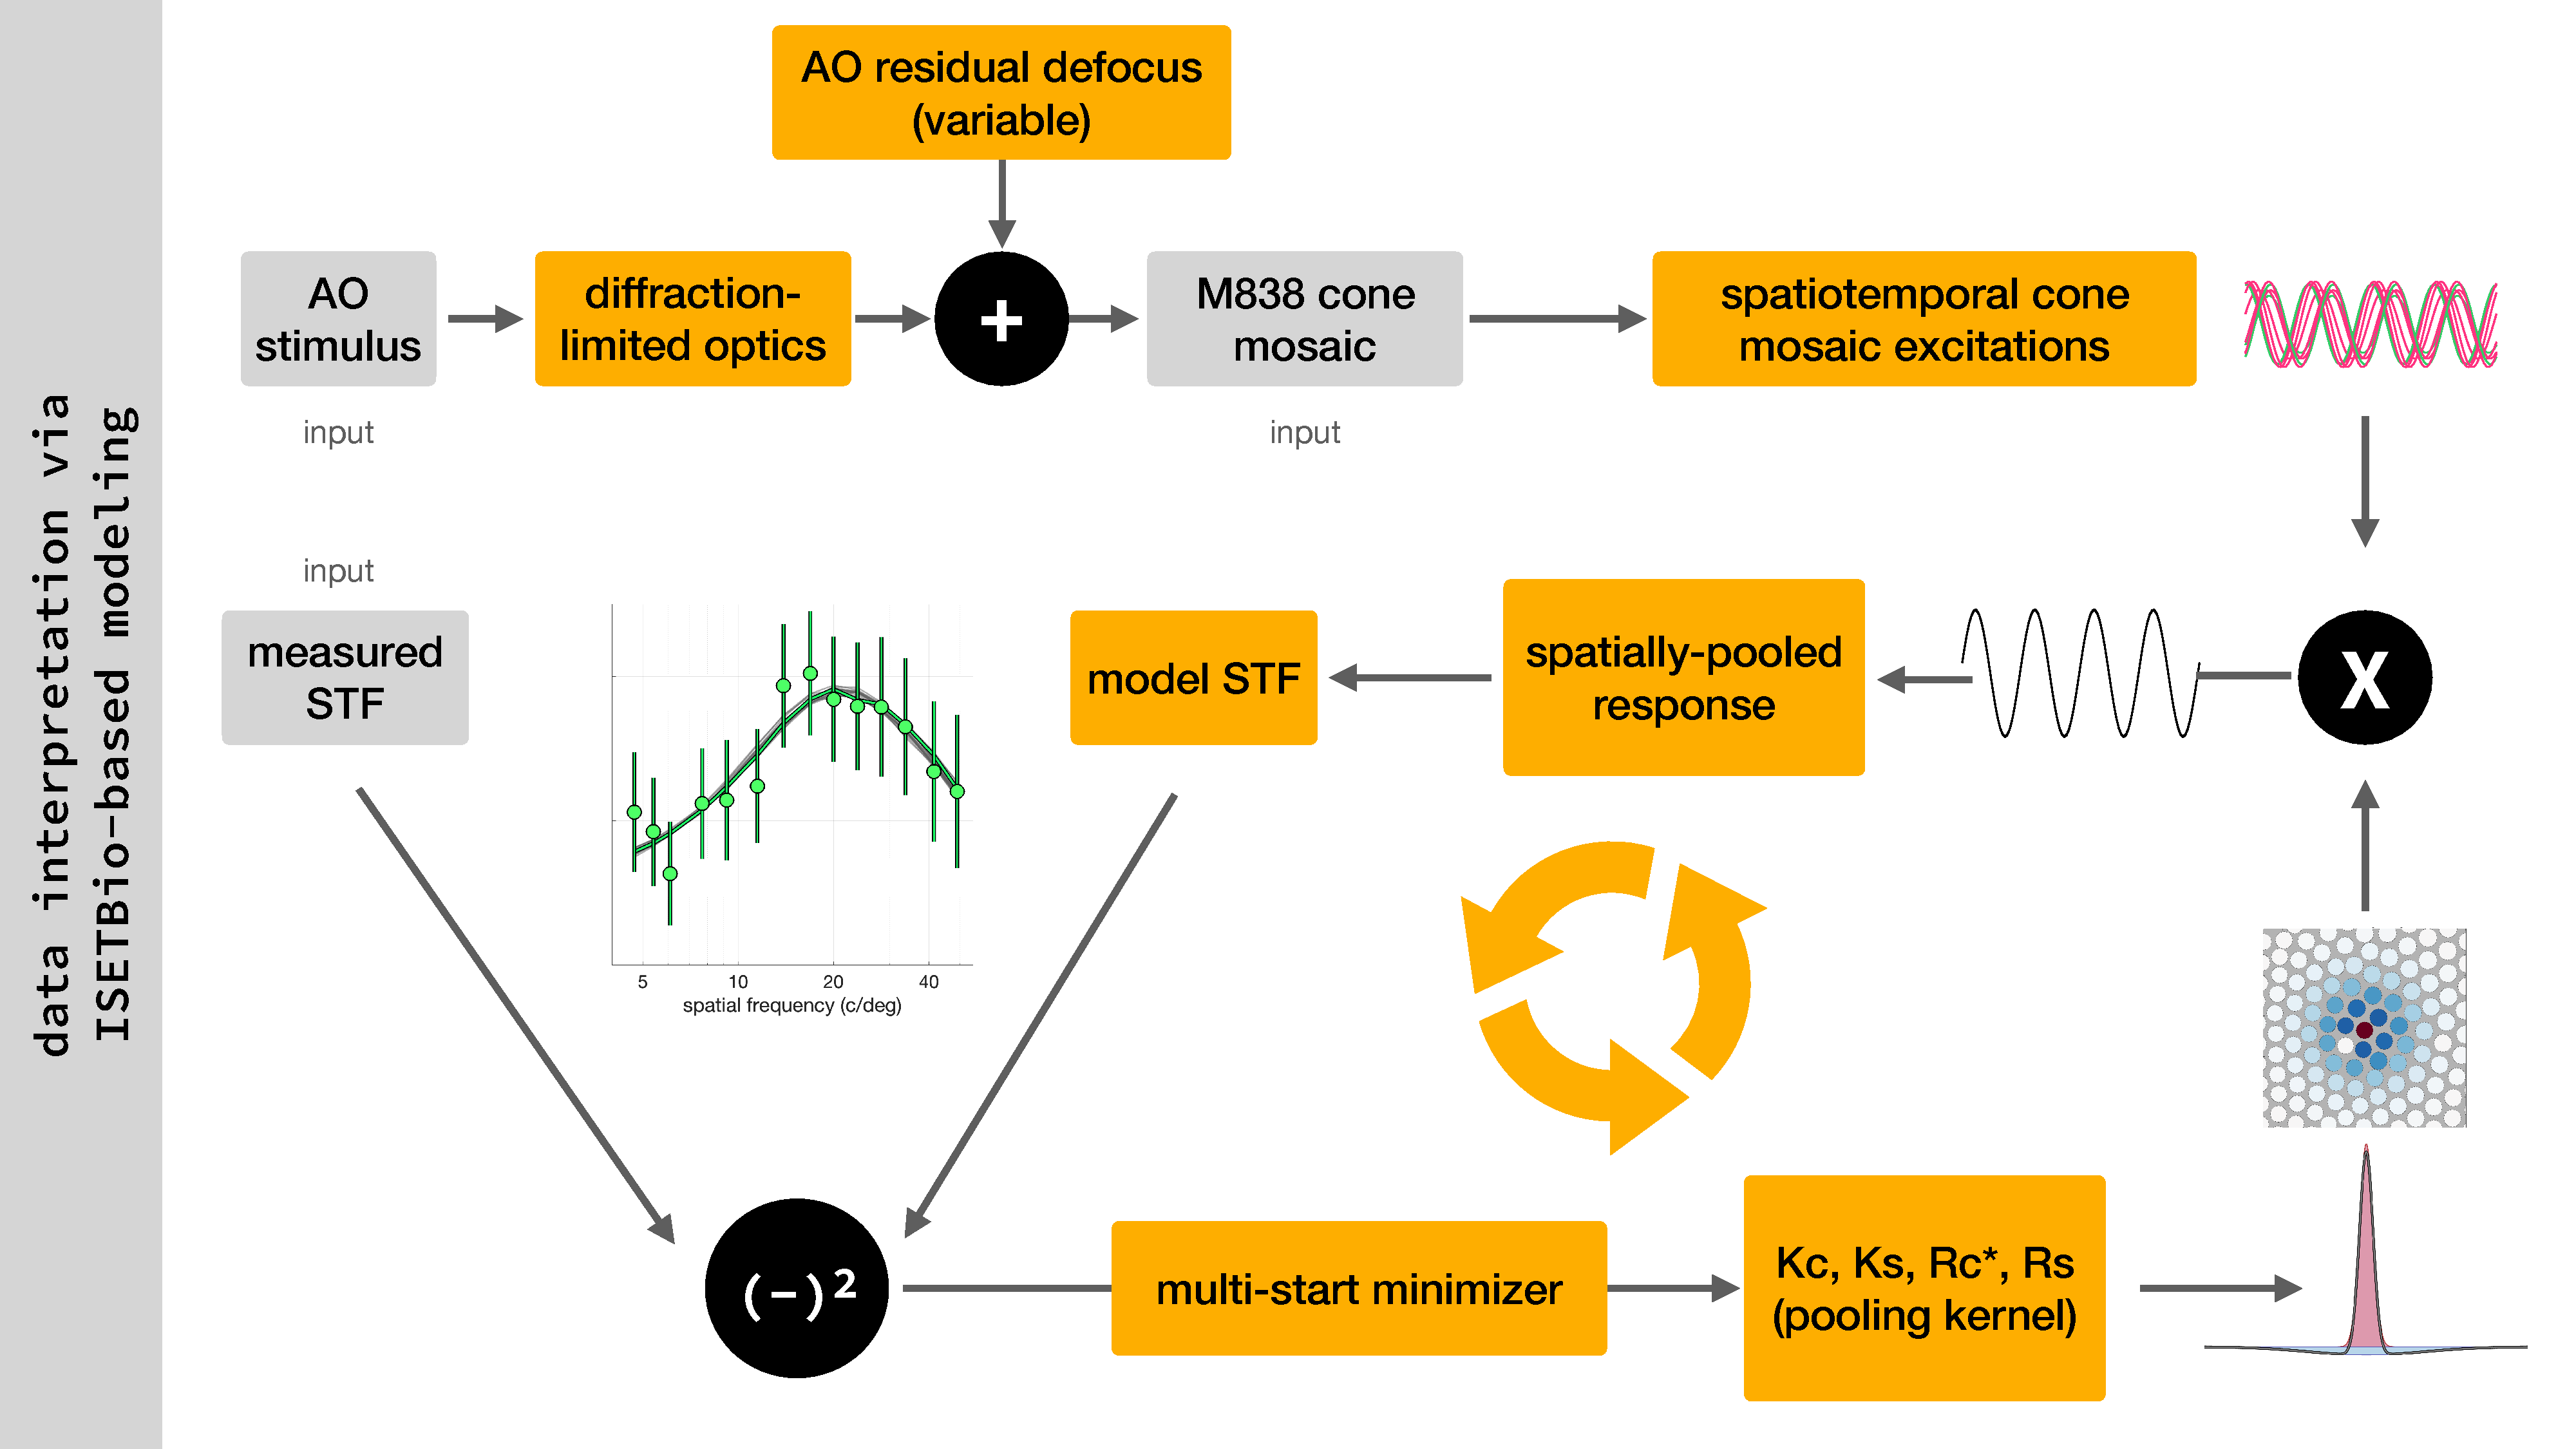
\includegraphics[width=7in]{Figures/ModelOverview.pdf} 
   \caption{Schematic overview of the ISETBio computational model.}
   \label{fig:ModelOverview}
\end{figure}


\begin{figure}[htbp] %  figure placement: here, top, bottom, or page
   \centering
   \includegraphics[width=7.5in]{Figures/Figure_Variabilities.pdf} 
   \caption{\textbf{Variability in estimating spatial distribution of cone weights from fitting models to the measured STF}. \textbf{A}. Variability due to assumed position of the recorded RGC receptive field (RF). \textbf{B.} Variability due to different recording sessions. \textbf{C}. Variability due to the different examined model scenarios. Figure format for all panels is as follows. The weights of cones feeding into the RF center are color coded in red in \textbf{Aa}. The weights of cones feeding into the RF surround are color-coded in blue in \textbf{Ab}. Horizontal slices through the RF center (red) and the RF surround (blue), computed by integrating over the y-dimension, the spatial profile on the input cones (cone aperture profile multiplied by the corresponding cone weight to the RF) are depicted in \textbf{Ac}. The measured fluorescence-based spatial transfer functions, which the computational model is fit to, $\mbox{STF}^{\Delta F / F}_{s_{test}}(\omega)$ (green disks), and the STF of the best-fit model, $\mbox{STF}^{m}_{s_{train}}(\omega)$ (orange line) are depicted in \textbf{Ad}.
}
   \label{fig:Variabilities}
\end{figure}


\begin{figure}[htbp] %  figure placement: here, top, bottom, or page
   \centering
   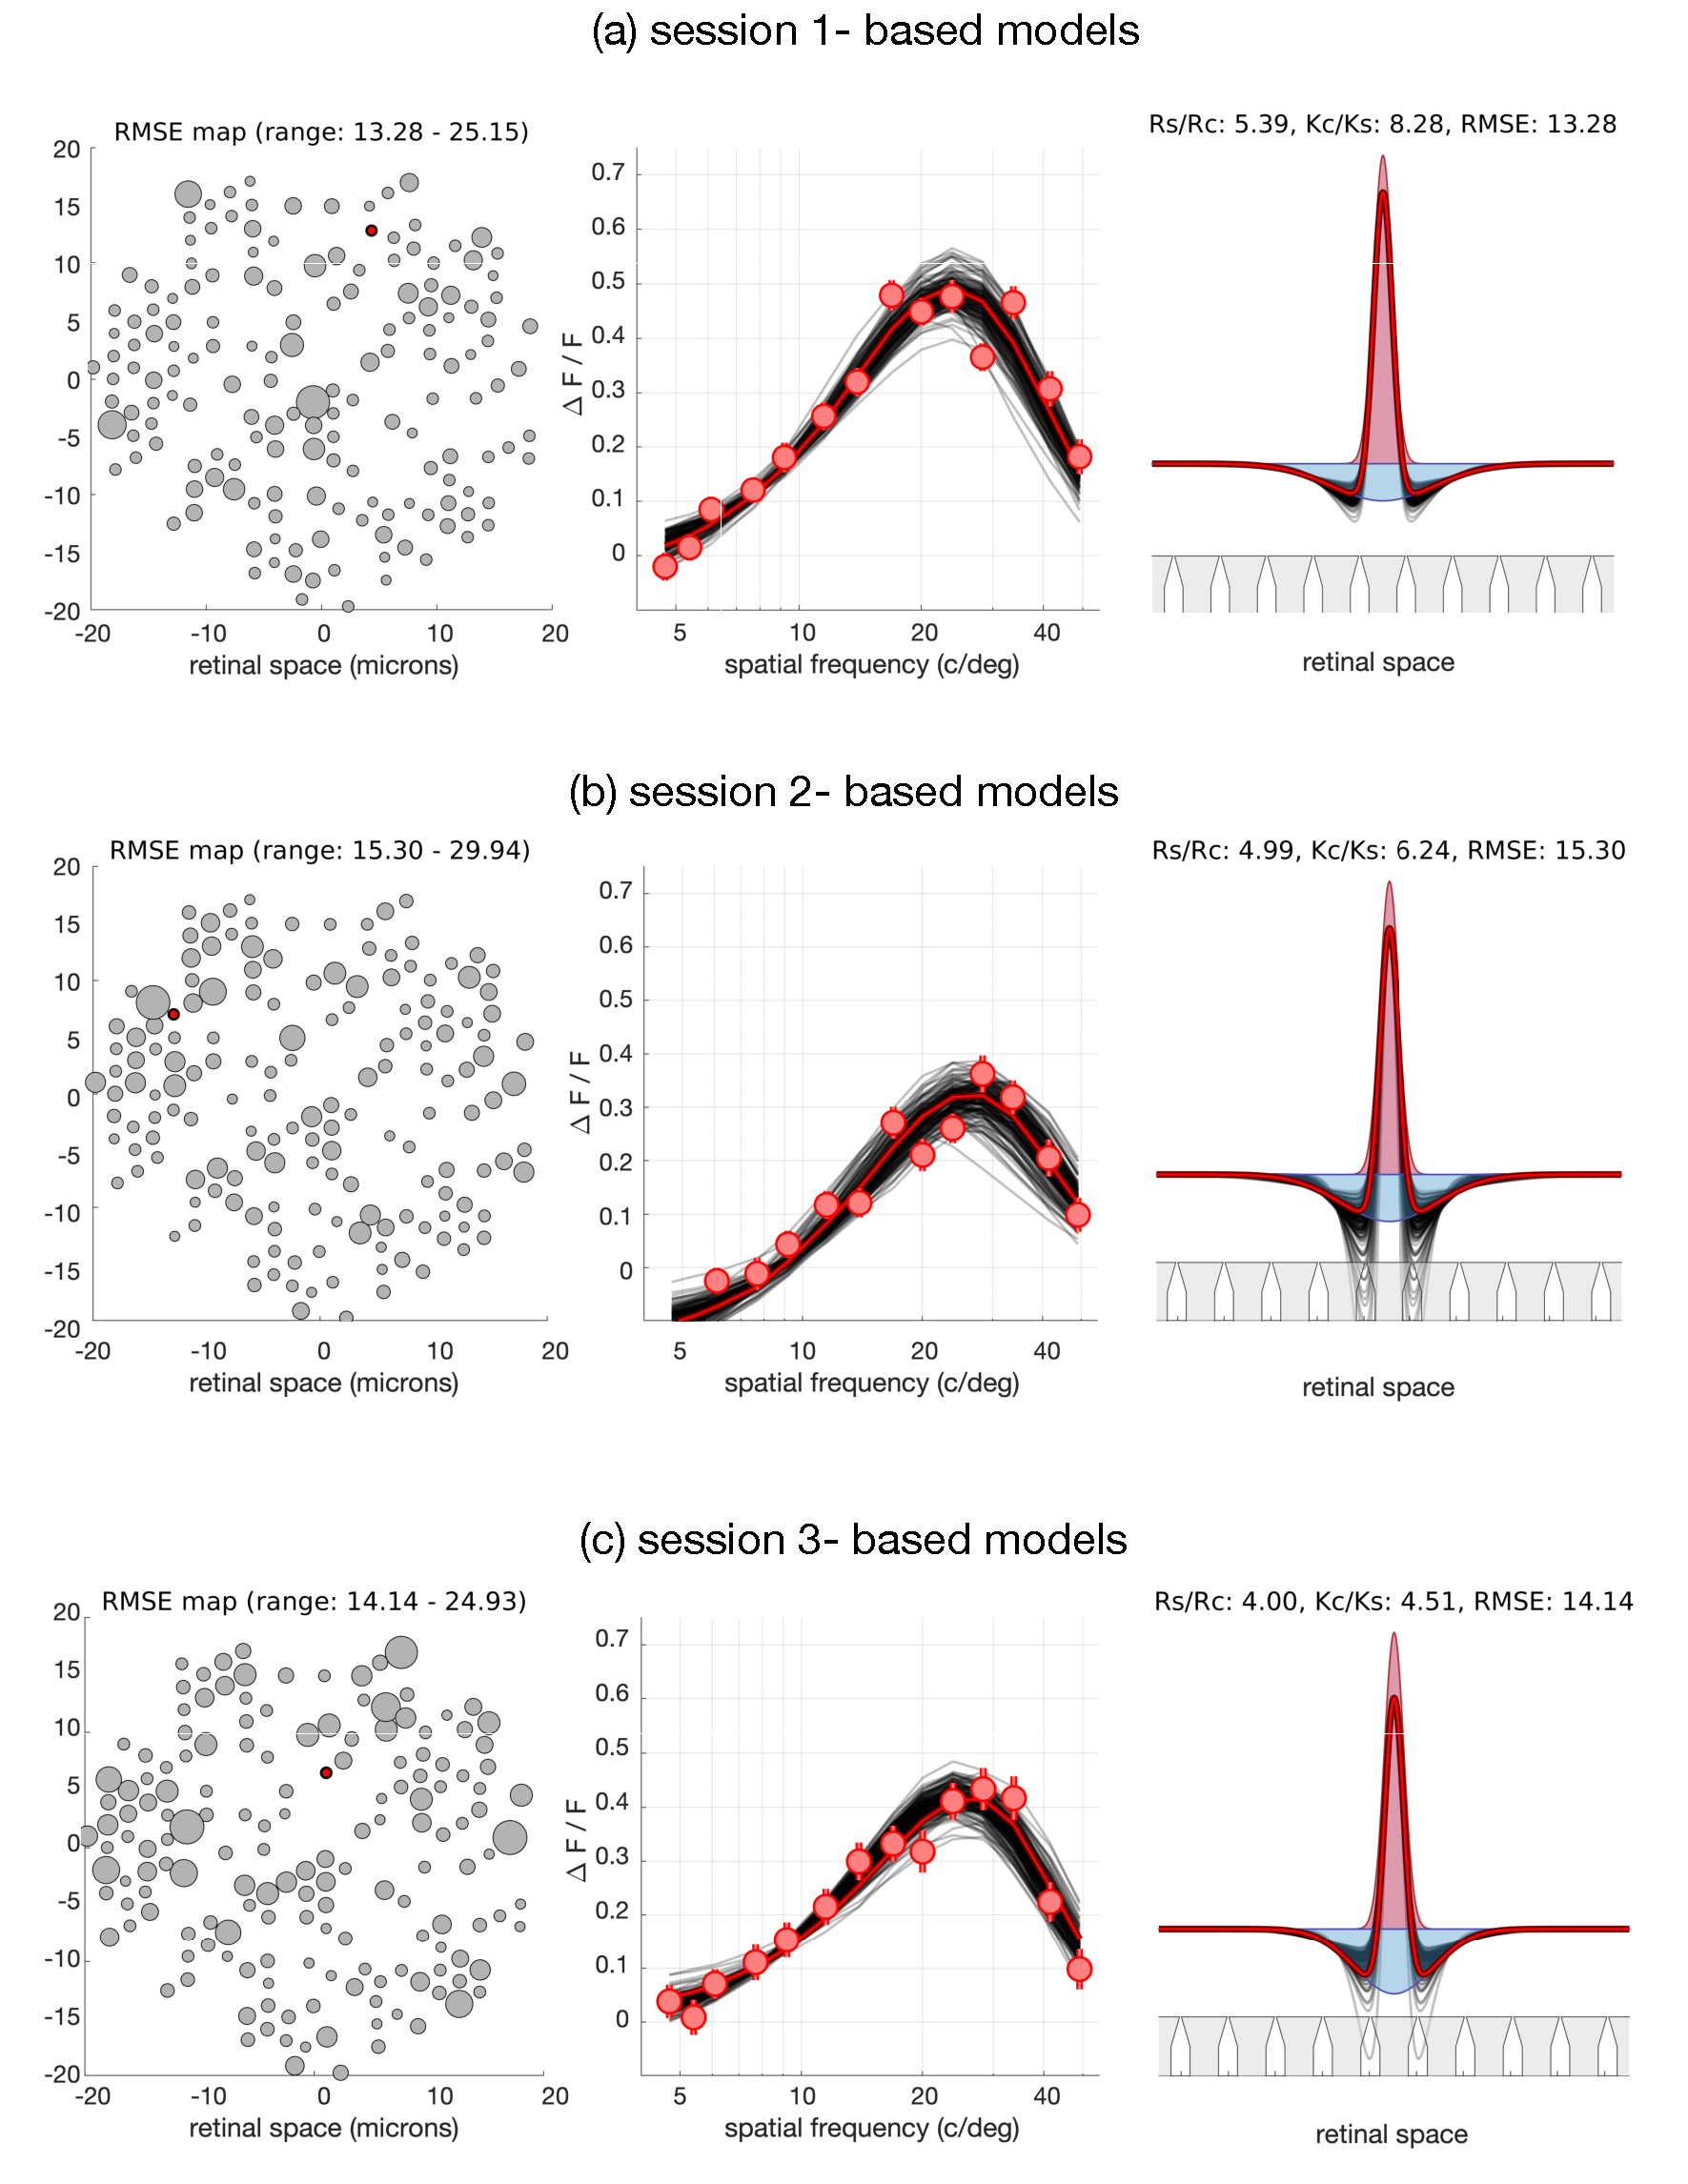
\includegraphics[width=6in]{Figures/CrossValidationMethod_TrainingModels.pdf} 
   \caption{Training RF models for an L-cone center RGC based on STF data recorded during the first (\textbf{A}), second (\textbf{B}) and third (\textbf{C}) recording session. \textbf{Left panels}: spatial map of RMSE between model STF and measured STF, as a function of center cone position in the examined model. There are a total of 161 models, each centered on one of 161 cones within the mosaic. Bubble size denotes magnitude of RMSE for each model. \textbf{Middle panels}: Fits of model STF (black lines) to the measured STF data (red disks) for all 161 examined models. The red line represents the best fit. \textbf{Right panels}: Black thin traces depict the RF profiles of the 161 examined models. The red thick line depicts the RF profile of the best fit model, whereas the pink and blue shaded areas depict the center and surround mechanism profiles of the best fit model. The apertures of cones are depicted schematically in gray.}
   \label{fig:CrossValidationApproach_TrainingModels}
\end{figure}

\begin{figure}[htbp] %  figure placement: here, top, bottom, or page
   \centering
   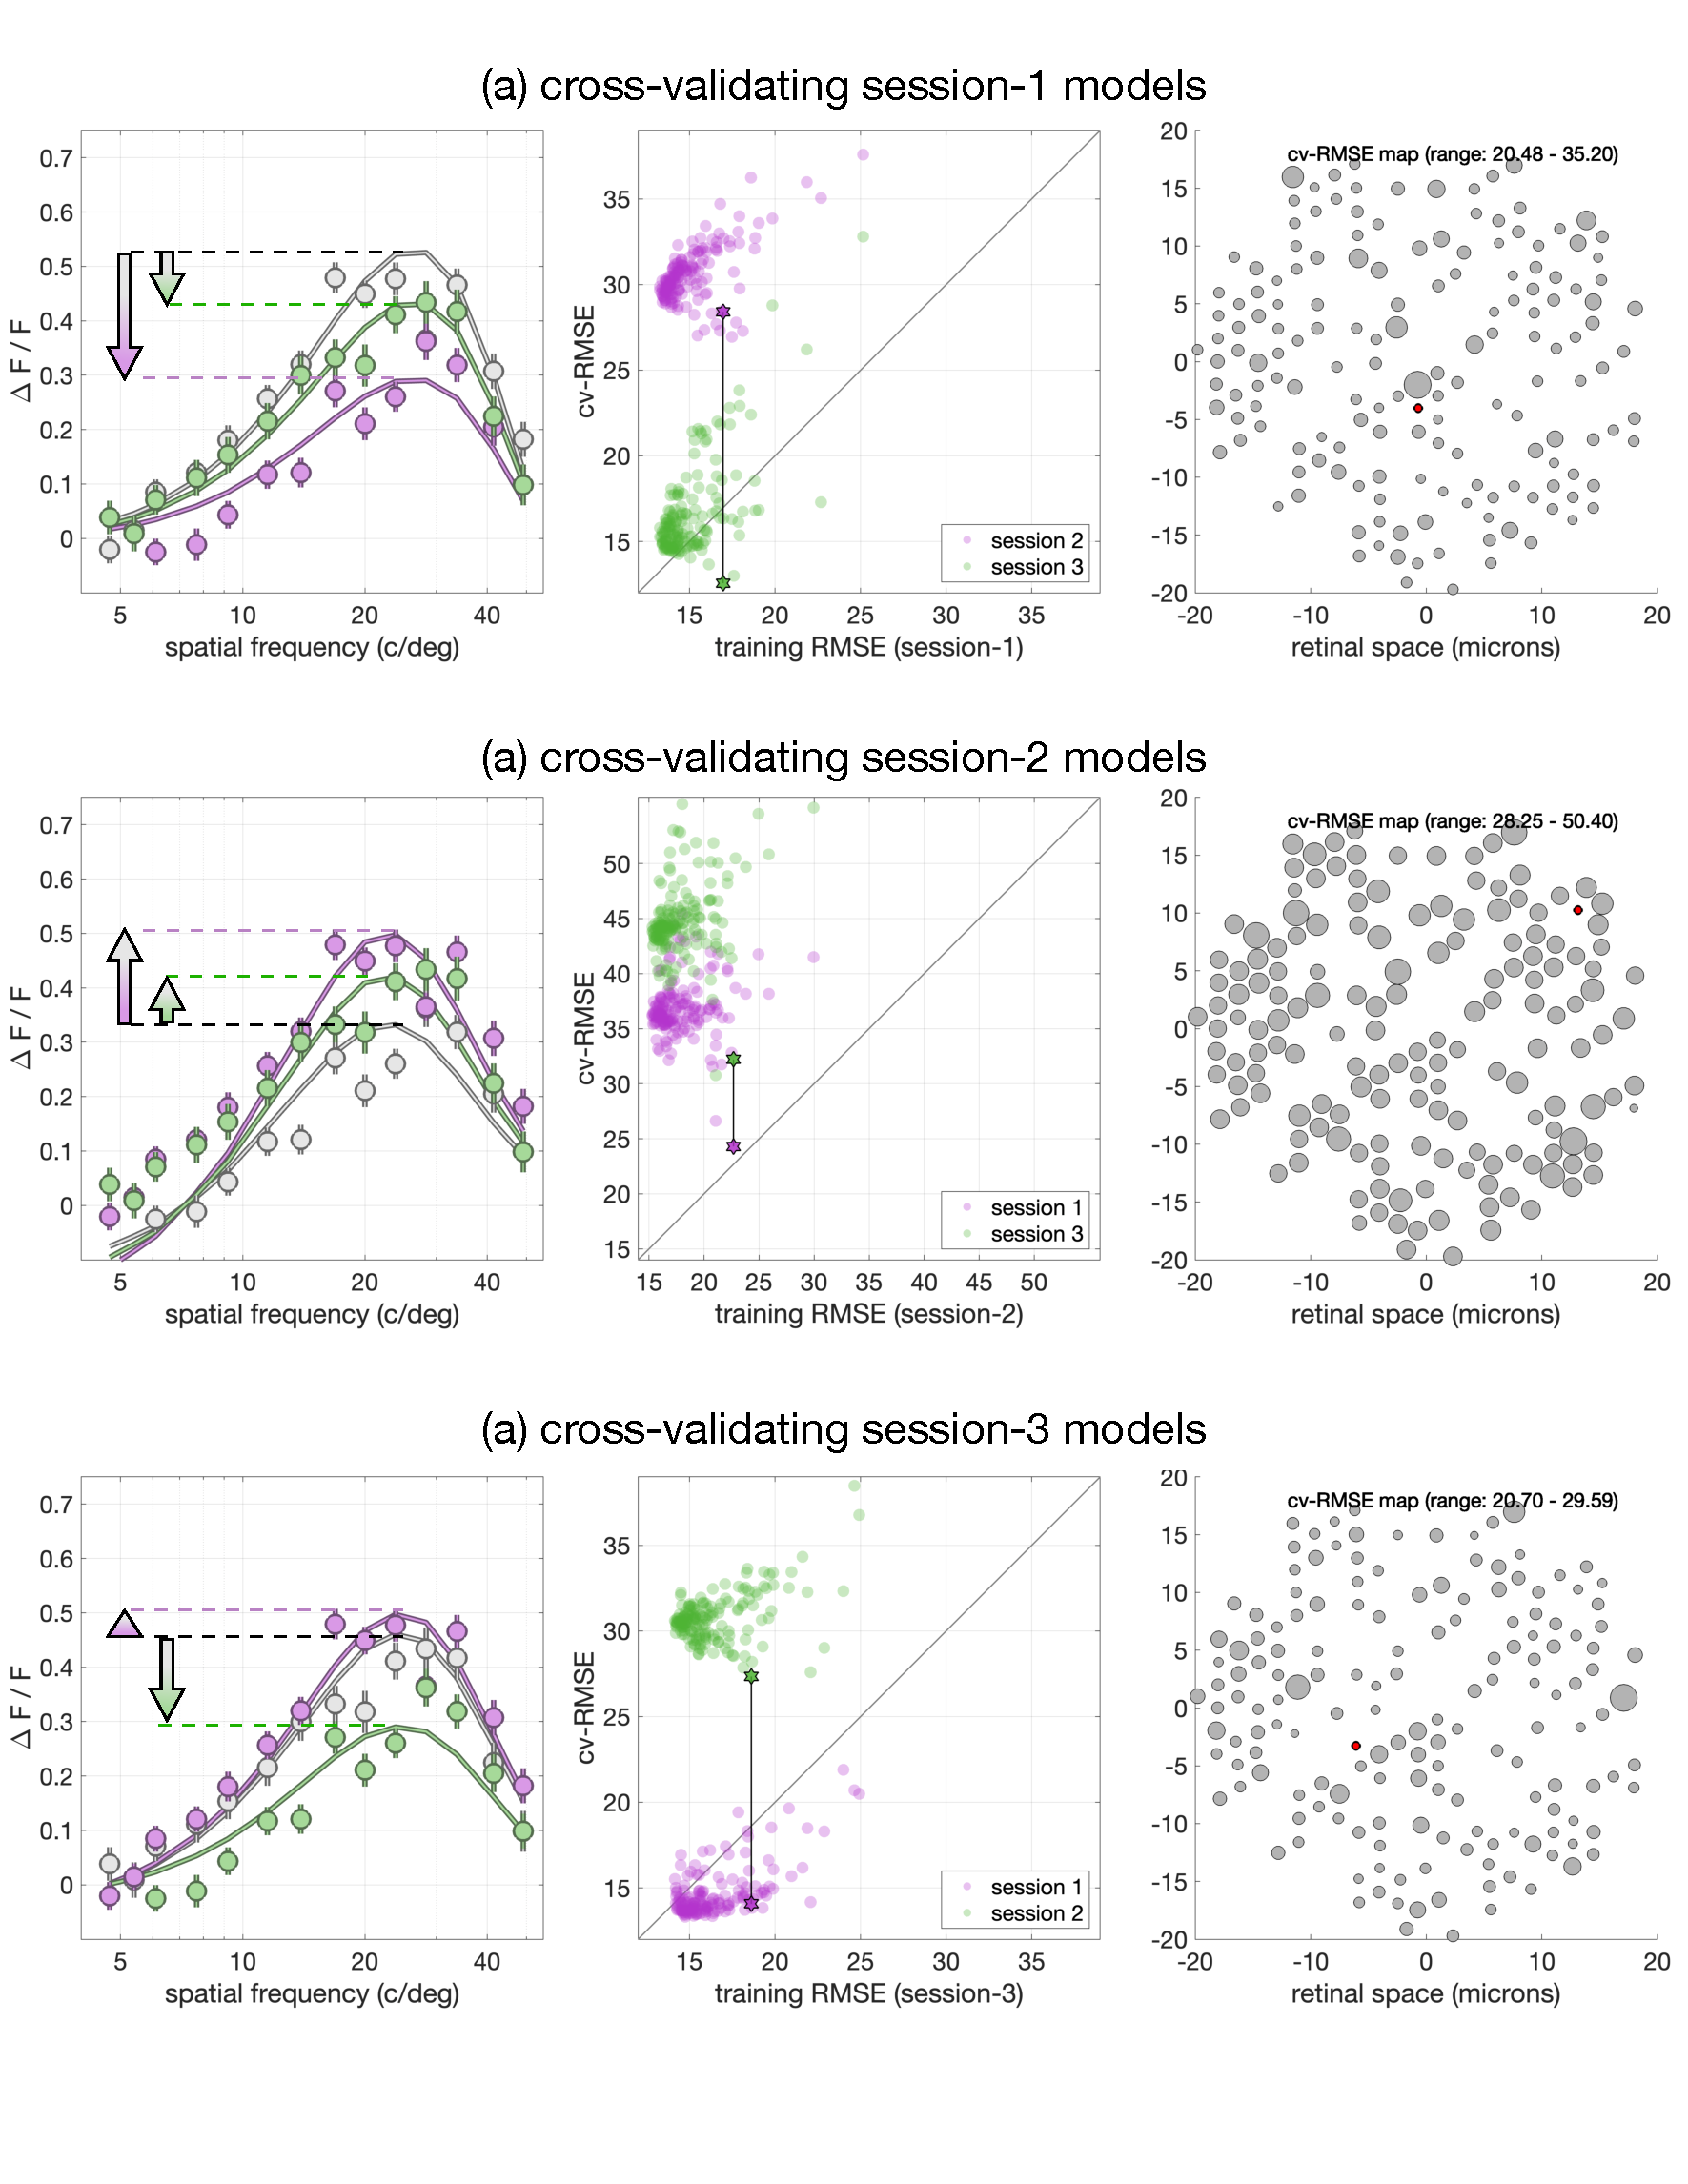
\includegraphics[width=6in]{Figures/CrossValidationMethod_CrossValidatingSession1Models.pdf} 
   \caption{Cross-validating RF models for the same L-cone center RGC cell. The model RF is trained on STF data recorded during the first recording session (\textbf{A}), the second session (\textbf{B}) and third session (\textbf{C}). \textbf{Left panels}: Gray lines depict the STF of the model RF trained in the current session that resulted in the minimum combined cross-validation error over the remaining 2 sessions, across all examined cone positions. Green and purple lines, depict the optimal cross-validated fits along with the scaling factor (arrows) that had to be applied to derive them from the STF of the model RF.  \textbf{Middle panels}: The cross-validated errors are plotted against the training errors for all examined cone positions. The connected stars indicate where the minimum combined cross-validated error occurred. \textbf{Right panels}: Spatial map of cross-validated errors, with bubble size indicated the error magnitude. The position of the cone at which this minimum occurred is denoted by the red circle.
    }
 \label{fig:CrossValidationApproach_CrossValidatingModels}
\end{figure}


\begin{figure}[htbp] %  figure placement: here, top, bottom, or page
   \centering
   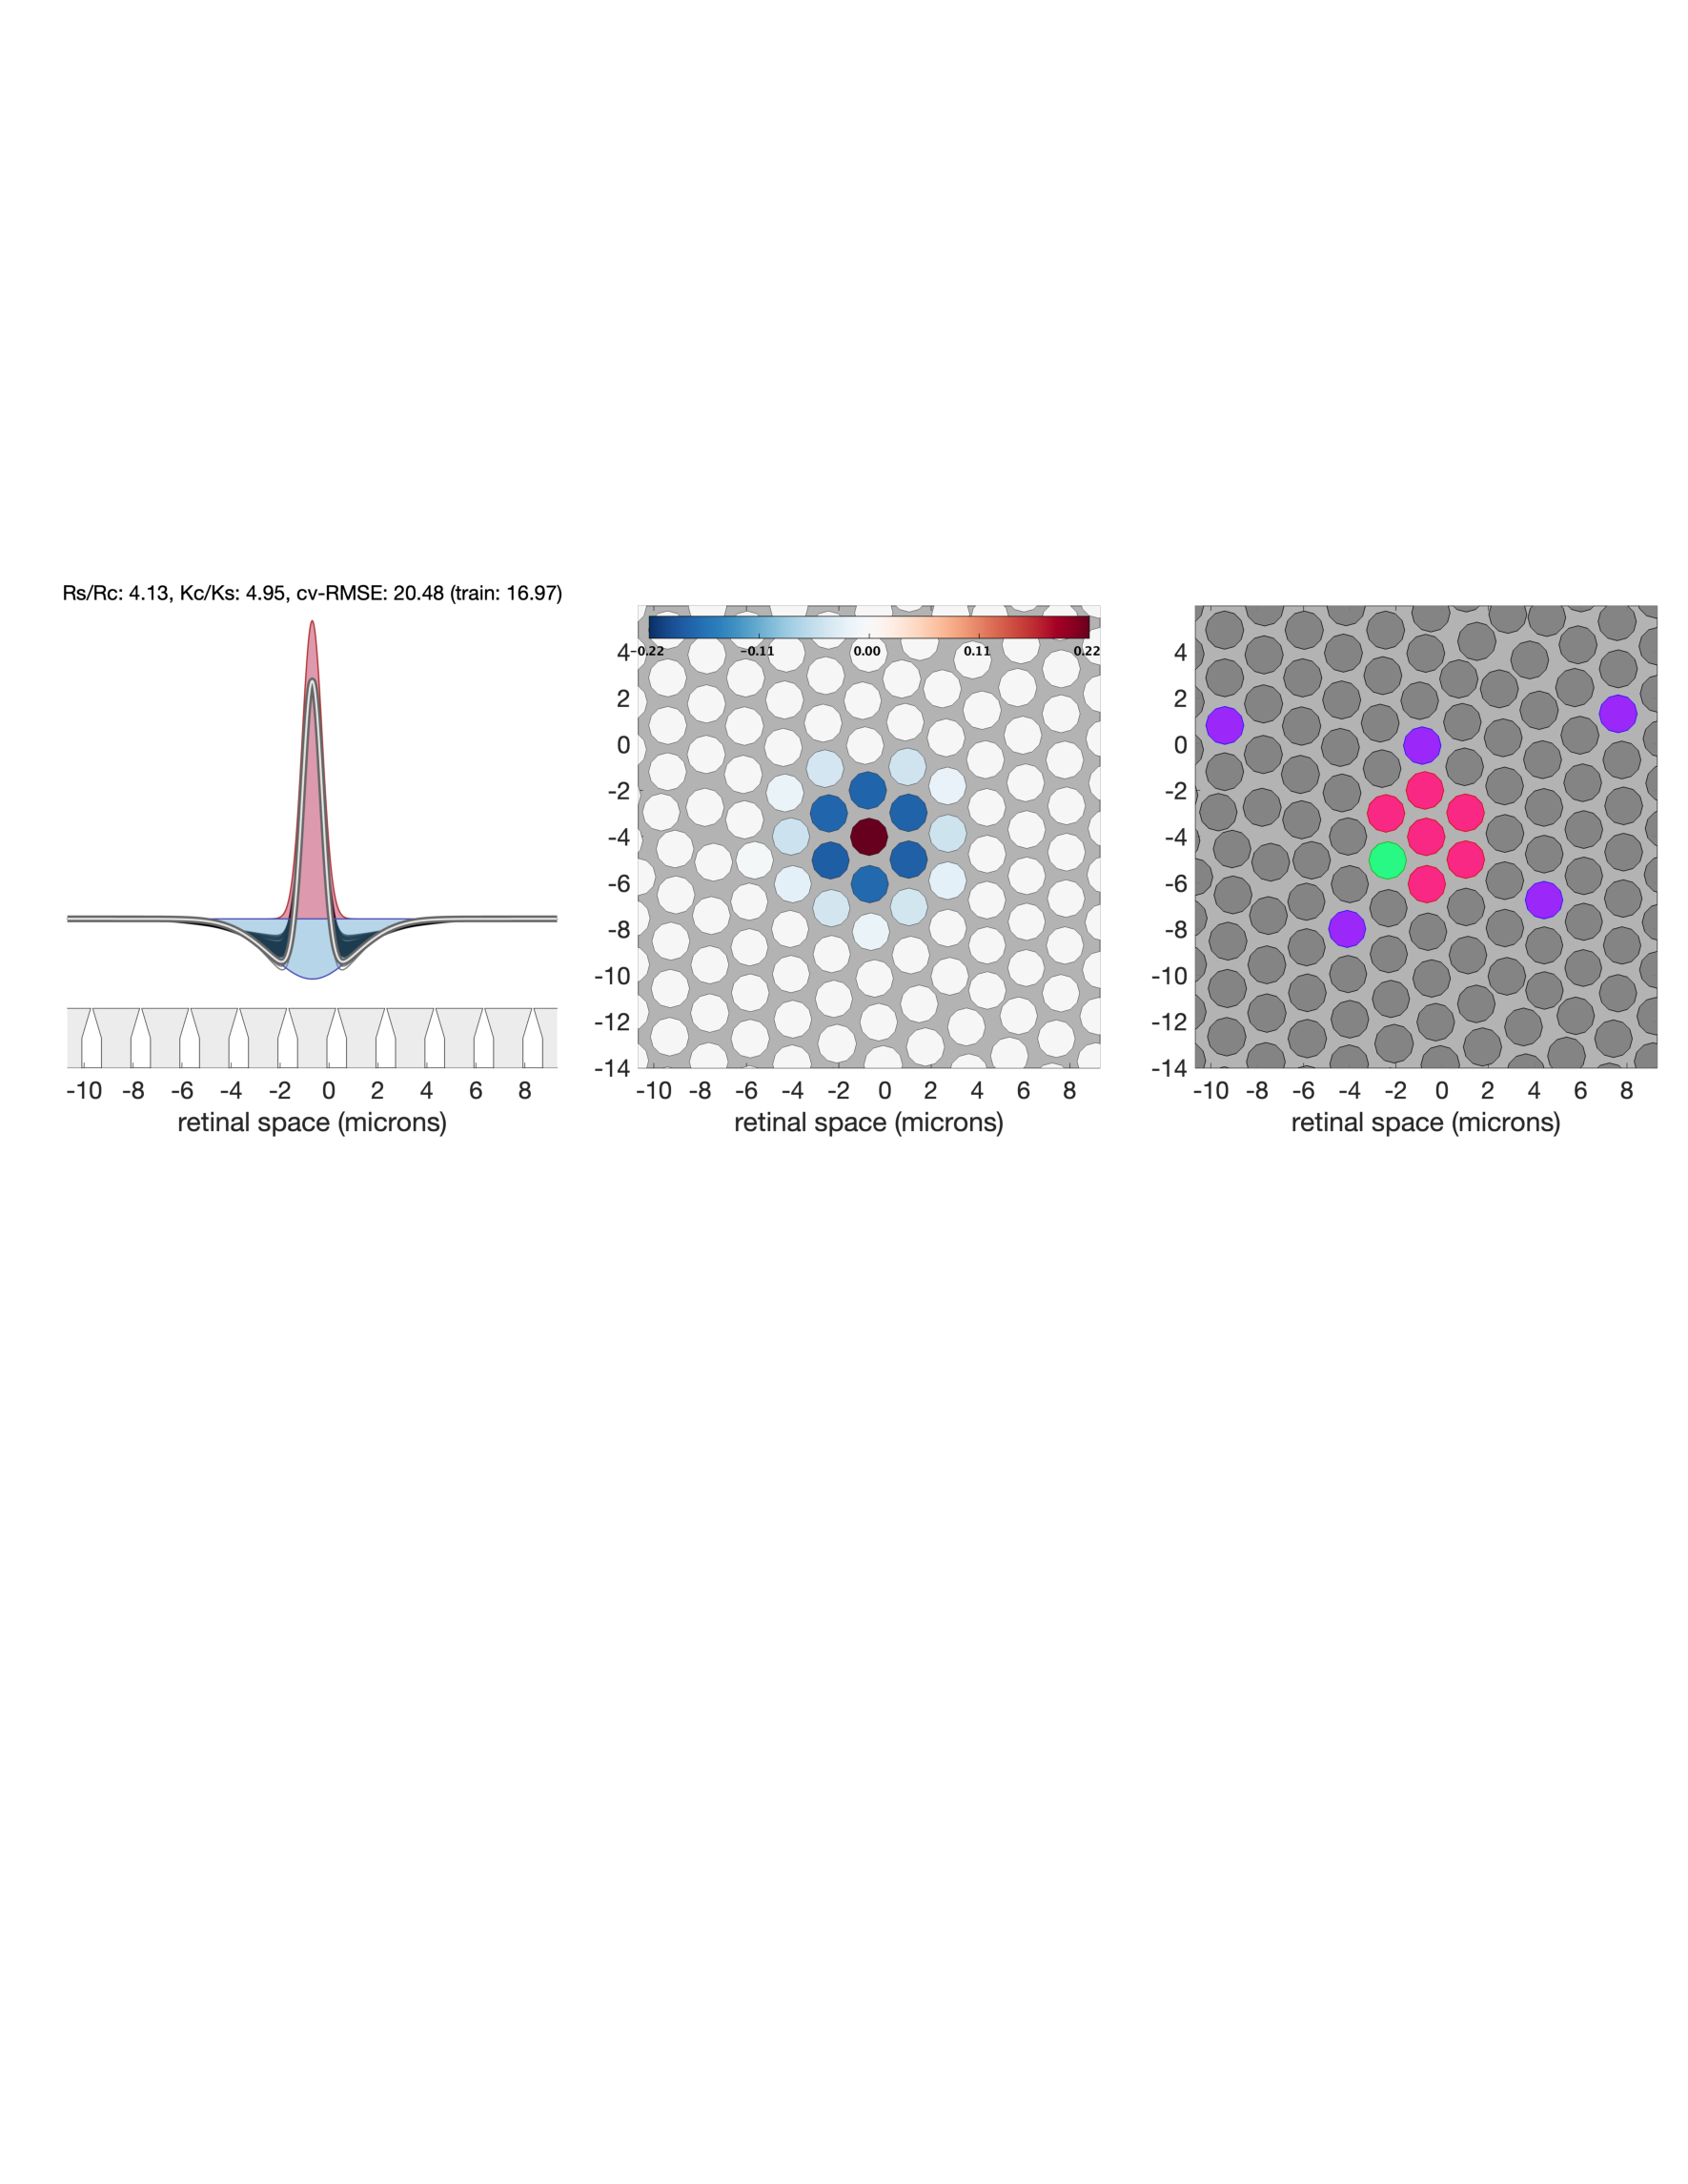
\includegraphics[width=6in]{Figures/CrossValidationMethod_BestCrossValidatedModel.pdf} 
   \caption{Best cross-validated RF model. \textbf{Left panel :} The RF profile of the best fit model, is depicted by the white thick line, whereas the pink and blue shaded areas depict the profiles of the center and surround mechanisms, respectively. Cone apertures are depicted schematically in gray below.  \textbf{Middle panel:} Weights of cones feeding into the RF center (red) and the RF surround (blue) mechanisms. \textbf{Right panel:} Labeling of L/M- (red/green) cones whose weights to the best cross-validated RF model are greater than 5\% of the center cone weight, or are S-cones (blue).
   }
 \label{fig:CrossValidationApproach_BestCrossValidatedModel}
\end{figure}

\newpage
\newpage





\end{document}  